\newpage
\section{WBS e Prospetto di Gantt}

Per sostenere al meglio le varie fasi di progetto, garantendone la maggior efficienza e la miglior gestione possibile, abbiamo adottato la seguente struttura WBS.

\begin{figure}[ht!]
	\centering
	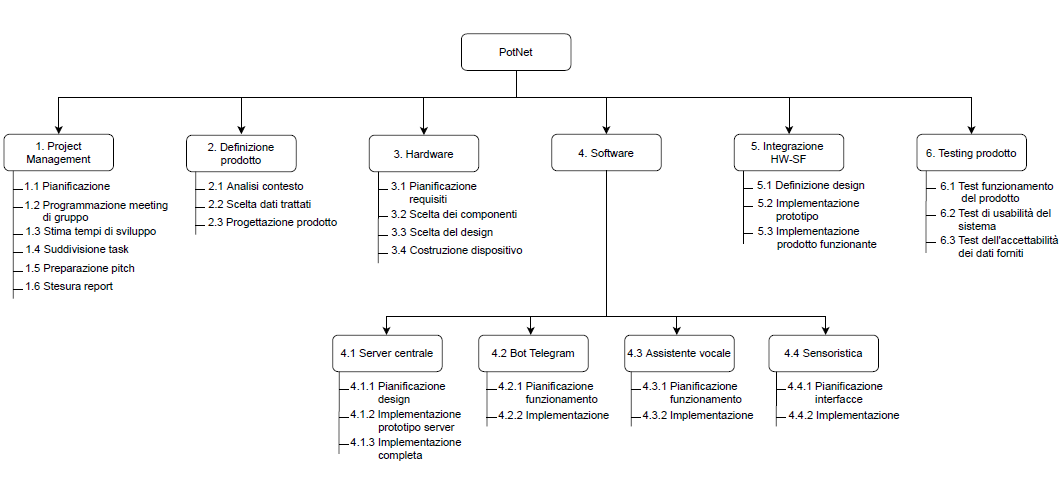
\includegraphics[width=\textwidth]{./images/wbs.PNG} 
	\caption{WBS del progetto PotNet \label{overflow}}
\end{figure}

Questa suddivisione delle attività di sviluppo di PotNet ci ha permesso di individuare tutte le attività chiave necessarie per la produzione di un prodotto finito.\\
Queste attività sono poi state inserite in un diagramma di Gantt per poterne gestire al meglio la suddivisione tra i vari membri del team affinché l'intero progetto sia portato a termine raggiungendo tutti gli obiettivi tecnici, temporali e di costo.

\begin{figure}[ht!]
	\centering
	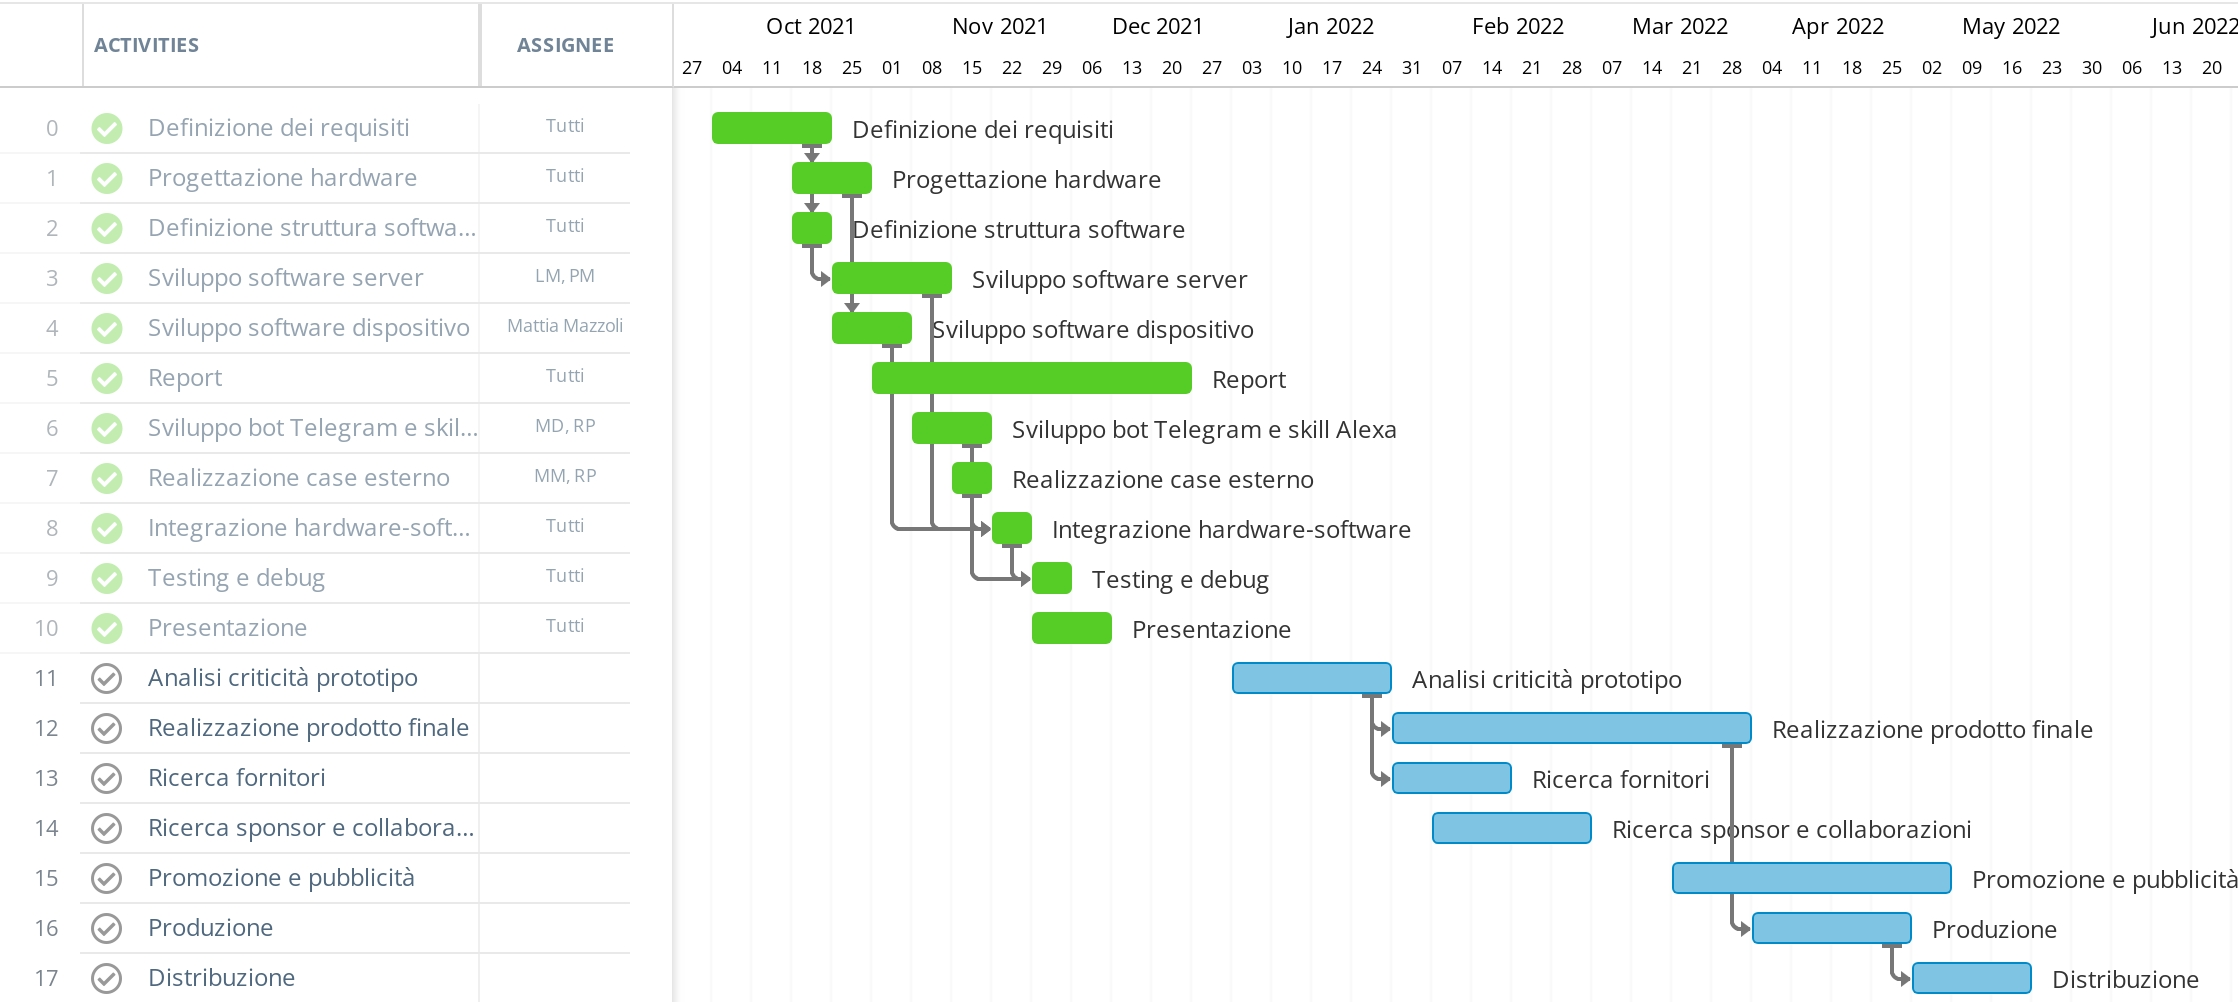
\includegraphics[angle=0,origin=c,width=\textwidth]{./images/Gannt.PNG} 
	\caption{Diagramma di Gantt del progetto PotNet \label{overflow}}
\end{figure}

\newpage
\theendnotes